\chapter{Background}
\label{ch:background}

% Describe protocols and systems your work depends on.
% In almost all cases, this should contain a section on SCION.

% Started in 2009 (15y ago)
% The SCION Internet became operational in 2017

This chapter provides important background information on the SCION Internet architecture, which is the main components of this security analysis.
It starts by introducing SCION and its core concepts and services, as well as its control and data plane.
Additionally, some security aspects of SCION and the proprietary SCION version provided by the company Anapaya are discussed.
In \cref{sec:security_testing}, we will explore different security testing methods and tools that are used to identify vulnerabilities in systems.


\section{SCION}

SCION \cite{Perrig2022} is a clean-slate Internet architecture focused on scalability, control and isolation and is designed to provide security, flexibility, and performance improvements over the current Internet.
This section delves into the fundamental concepts of SCION, offering detailed explanations of its control and data planes and highlighting its key security mechanisms.
Additionally, we will also briefly introduce Anapaya, the company that provides SCION services.

Unless otherwise stated, the background information presented here is primarily based on  ``The Complete Guide to SCION'' \cite{Perrig2022}.

\subsection{Core Concepts}
In the following we explain SCION's core features and how it achieves them.
\subsubsection{Isolation}

By grouping different autonomous systems (ASes) into isolation domains (ISDs), as shown in \cref{fig:scion_isd_architecture}, SCION provides both fault and trust isolation.
Each ISD contains core ASes that administer the ISD, form the root of trust of the ISD, and provide connectivity to other ISDs.
The configuration of an ISD is stored in a signed file called trust root configuration (TRC), which includes for example root certificates or policies.
If a misconfiguration occurs in an ISD, only that ISD is affected and the rest of the Internet can continue to operate.

\begin{figure}[h]
    \centering
    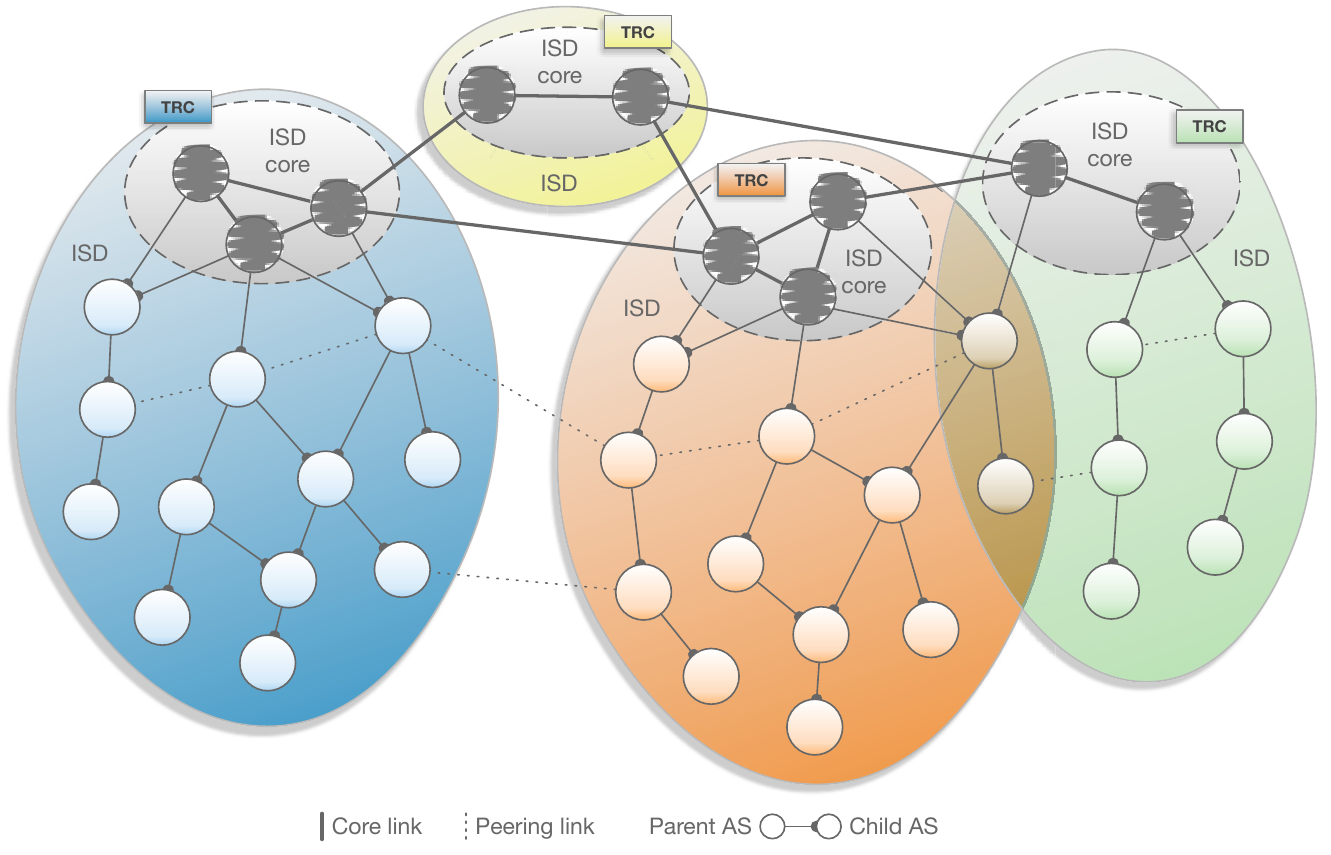
\includegraphics[width=0.75\textwidth]{figures/scion_isd_architecture.png}
    \caption{SCION Architecture with ISD and ASes. ASes are represented by circles. Figure taken from Chapter 2 of the SCION book \cite{Perrig2022}.}
    \label{fig:scion_isd_architecture}
\end{figure}


\subsubsection{Control}

SCION allows users to request and select the optimal paths for their network traffic to reach the desired destinations.
A network path can contain up to three path segments, called up-, core- and down-segment.
The up-segment is the path from the source to its core AS, the core-segment is the path between core ASes and the down-segment is the path from the destination core AS to the destination.
These segments are combined to form a path that the packets will traverse.
This allows users to avoid certain regions or countries they do not trust and that may perform some sort of traffic analysis.

Users are not limited to a single path.
With the option to utilize multiple paths simultaneously, SCION empowers users with greater control and flexibility over their network traffic.
This multipath feature also ensures higher availability in case of a network issue along a path.


\subsubsection{Scalability}

The path information in SCION packets is stored in the SCION packet header.
Based on this information, the SCION routers can forward the packets to the next hop without storing any state information or performing expensive longest prefix matching as traditional IP routers do.
The concept of ISD impacts also the scalability of SCION.
It allows splitting up the routing processes into two levels:
One for routing within an ISD and one for routing between ISDs.


\subsection{Services}
This section discusses the main services of SCION.

The \textbf{border router} sits at the edge of an AS and forwards outgoing SCION packet to neighboring remote ASes or incoming packets within the local AS.
To support legacy end hosts that are not able to communicate over SCION, the \textbf{SCION-IP gateway (SIG)} is used.
It translates SCION packets to IP packets and vice versa.
SCION-enabled end host run the \textbf{SCION daemon} and the \textbf{SCION dispatcher}.
The dispatcher is responsible for sending and receiving SCION packets, whereas the main task of the daemon is to fetch path information.

The \textbf{control service} is generic term for the following other services that run in an AS:
The \textbf{beacon service} is responsible for path exploration and the \textbf{path service} for path registration, as well as providing path lookup services to end hosts.
Key management and signature validation is done by the \textbf{certificate service}.


\subsection{Control Plane}
\label{sec:control_plane}

The control plane in SCION is responsible for discovering network path segments.
These segments are verified using AS certificates.
In the following, path exploration and its security mechanisms are explained.
For simplicity, we will only focus on control plane packets within an ISD and not between core ASes of different ISDs.
The interested reader can find more information in Chapter 4 of the SCION book \cite{Perrig2022}.

\subsubsection{Path Exploration}
Path segments are discovered by using path-segment construction beacons (PCBs).
These are special control plane packets that are always originated by a core AS and subsequently propagated to non-core child ASes.
During this traversal, PCBs gather information about the path (e.g. the crossed interfaces at the border routers) and the ASes traversed.
Within an AS, the beacon service verifies the structure and authenticity of the PCB.
If the PCB is validated successfully, it stores the PCB in its local database.
The beacon service then selects the best combination of PCBs and forwards them to the beacon service in a next AS, thereby continuing path exploration.
This process, known as beaconing, is depicted in \cref{fig:scion_path_exploration}.

\begin{figure}[h]
    \centering
    \includegraphics[width=0.75\textwidth]{figures/scion_beacon.png}
    \caption{Propagation of PCBs within an AS. Figure taken from Section 2.3.1 of the SCION book \cite{Perrig2022}.}
    \label{fig:scion_path_exploration}
\end{figure}

\subsubsection{PCB Format}
Formally, a PCB is structured as follows:
$$ PCB = \langle INF \parallel ASE_0 \parallel ASE_1 \parallel \ldots \parallel ASE_n \rangle $$

The PCB comprises an info field $INF$ and a series of AS entries $ASE_i$, where each $ASE_i$ contains all path-related information for the $i$-th traversed AS.
The info field is defined as:
$$ INF = \langle Flags_{INF} \parallel SegID \parallel TS \rangle $$

Here, $Flags_{INF}$ represents various flags used primarily in the data plane during packet forwarding, $SegID$ is a random segment ID, and $TS$ denotes the timestamp indicating when the PCB was created.

For the AS entry, we use a simplified format to highlight the key fields.
A detailed description of the full format can be found in Section 4.1.1.2 of the SCION book \cite{Perrig2022}.
The simplified AS entry format includes of a hop field $HF$ and a signature $\Sigma$.
The format of the hop field is as follows:
$$ HF = \langle Local \parallel Next \parallel Flags_{HF} \parallel ExpTime \parallel ConsIngress \parallel ConsEgress \parallel HFAuth\rangle $$

$Local$ is the ISD-AS identifier of the AS, $Next$ is the ISD-AS identifier of the next AS in the path (i.e. where the PCB is forwarded next).
$Flags_{HF}$ indicates different processing options for the AS.
The $ExpTime$ field specifies for how long the hop field is valid.
The ingress and egress interfaces (in direction of construction/beaconing) are stored in $ConsIngress$ and $ConsEgress$ respectively.
The hop field is authenticated using the $HFAuth$ field, which is a message authentication code (MAC).
In \cref{sec:mac_calc} we will explain how this MAC is calculated and used.

The signature field $\Sigma$ is used to authenticate the AS entry and is calculated using the private key $K_i$ associated with the AS's public key, which is validated by the certificate of the AS.
The signature is computed over the info field, all previously traversed AS entries, and the current hop field, or formally expressed as:
$$\Sigma_i = \text{Sign}_{K_i} \bigl( INF \parallel ASE_0 \parallel \dots \parallel ASE_{i-1} \parallel HF_i \bigr)$$

\subsubsection{MAC calculation}
\label{sec:mac_calc}
As previously mentioned, the $HFAuth$ value authenticates the hop field.
This section illustrated how the MAC value also authenticates all previously traversed hops.

Consider a PCB traversing the ASes $AS_0, \dots, AS_n$ with their corresponding secret keys $K_0, \dots, K_n$
The core AS $AS_0$ initiates the beaconing process by sampling a random value, i.e. the segment identifier:

$$ SegID = \beta_0 = Random() $$

Using this value, each AS computes its hop field MAC as follows:
\begin{align*}
    \sigma_i    &= \text{MAC}_{K_i}(\beta_i, TS, ExpTime_i, ConsIngress_i, ConsEgress_i) \\
    \beta_{i+1} &= \beta_i \oplus \sigma_i[0:16] \\
    HFAuth_i &= \sigma_i[0:48]
\end{align*}

Here, $\oplus$ denotes the bitwise XOR operation, and the notation $X[a:b]$ refers to the substring of $X$ from index $a$ (inclusive) to $b$ (exclusive), where the values represent the bit positions.
The hop field authenticator is truncated to 6 bytes to minimize communication overhead.
Additionally, only $\beta_0$ is stored in the $SegID$ field of the PCB, as the other $\beta_i$ values can be recomputed based on $\beta_0$ and the $HFAuth$ values of the previous hop fields.

Recalculation of these values during packet forwarding in the data plane would be too expensive.
Therefore, each router continuously updates the $SegID$ to reflect the value of $\beta_{i+1}$, which the next router uses to calculate its MAC value.

\subsubsection{Path-segment registration}
Path segments are derived from PCBs and must be registered first before they can be utilized by the end hosts.
From the stored PCBs, the up- and down segments get created:
Since these path segments start or end at the local AS, the selected PCB has to be modified accordingly:
The $Next$ field and the $ConsEgress$ field in the hop field are cleared, and afterwards, the MAC is recomputed on these modified PCBs.
The up-segments are forwarded to the local path service, while the down-segments are sent to the path service of the core AS that originated the PCB.

\subsubsection{SCION Control Message Protocol (SCMP)}


The SCION Control Message Protocol (SCMP) is analogous to ICMP and is used for reporting error and informational messages in SCION networks.
The different types of SCMP messages are shown in \cref{fig:scmp_message_types}.

\begin{figure}[h]
    \centering
    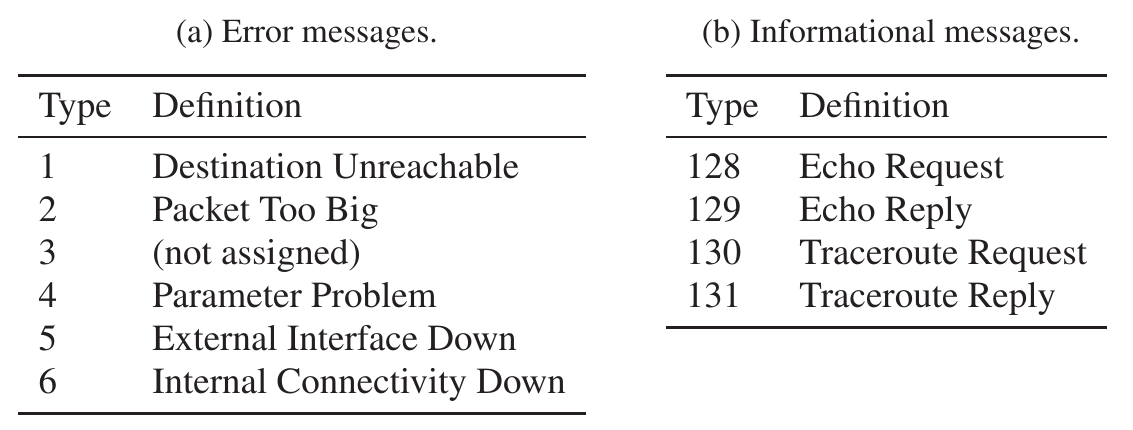
\includegraphics[width=0.75\textwidth]{figures/scmp_message_types.png}
\caption{Different types of SCMP messages. Original figure from the SCION book \cite[4.7.2]{Perrig2022}.}
    \label{fig:scmp_message_types}
\end{figure}

These messages deliver important information to end host, enabling actions such as network traffic optimization, path switching, and MTU modification.
Given that these messages can lead to significant decisions, their authentication is crucial.
The SCION specification mandates that all SCMP error messages must be authenticated with DRKey (see \cref{sec:drkey} for more details).
Authentication on SCMP informational messages is optional; however, responses must be authenticated if and only if the request was authenticated.

\subsection{Data Plane}
Delivering network packets in SCION between end hosts is managed by the data plane.
It is path-aware and utilizes the path information embedded in the packet header to forward the packets to the next hop.
This section first describes the packet format and subsequently addresses how the path header is constructed and reversed.
Finally, the processing steps at the routers are explained.

\subsubsection{Packet Format}
SCION packets contain a network-layer (layer 3) SCION header, which is structured as depicted in \cref{fig:scion_header_format}.

\begin{figure}[h]
    \centering
    \renewcommand{\arraystretch}{1.5} % Adjust the value to increase/decrease spacing
    \begin{tabularx}{0.5\textwidth}{|>{\centering\arraybackslash}X|}
        \hline
        Common header \\
        \hline
        Address header \\
        \hline
        Path header \\
        \hline
    \end{tabularx}
    \caption{SCION header format, based on Figure 5.2 of the SCION book \cite{Perrig2022}.}
    \label{fig:scion_header_format}
\end{figure}

The SCION common header includes fields needed to process the next headers including details such as header and packet length, the type of the path header, as well as the source and destination address types.

The address header contains the ISD and AS identifiers along with the host addresses of the source and destination.

The SCION path header specifies the path information required for packet forwarding.
We will only focus on the SCION path type, as it is the most common one.
Its structure is shown in \cref{fig:scion_path_header} and starts with a path meta header, 

$$ PathMetaHdr = \langle CurrINF \parallel CurrHF \parallel Seg0Len \parallel Seg1Len \parallel Seg2Len \rangle $$

followed by the info fields and hop fields.
The path meta header consists of the indices of the current info field $CurrINF$ and hop field $CurrHF$, as well as the lengths of the up-, core- and down-segments ($Seg0Len$, $Seg1Len$, $Seg2Len$ respectively).

\begin{figure}[h]
    \centering
    \renewcommand{\arraystretch}{1.5} % Adjust the value to increase/decrease spacing
    \begin{tabularx}{0.5\textwidth}{|>{\centering\arraybackslash}X|}
        \hline
        Path meta header \\
        \hline
        Info field (up) \\
        \hline
        Info field (core) \\
        \hline
        Info field (down) \\
        \hline
        Hop field \\
        \hline
        \cdots \\
        \hline
        Hop field \\
        \hline
    \end{tabularx}
    \caption{Structure of the SCION path header.
    Not all info fields must be present (at least one and at most all three), and their order is fixed.
    Based on Figure 5.5 of the SCION book \cite{Perrig2022}.}
    \label{fig:scion_path_header}
\end{figure}

The flags field in the info field include the $ConsDir$ single-bit flag, which indicates whether the corresponding path segment is traversed in the direction of construction (i.e. beaconing) or in the reverse direction.

\subsubsection{Path Construction and Reversal}

\cref{fig:scion_path_header_contruction} illustrates the construction of the path header from the individual path segments.
Following the path meta header up to three info fields are included.
Their order is fixed and corresponds to the info field of the up-, core-, and down-segments.
Subsequently, the hop fields are added in the order of the path segments.

\begin{figure}[h]
    \centering
    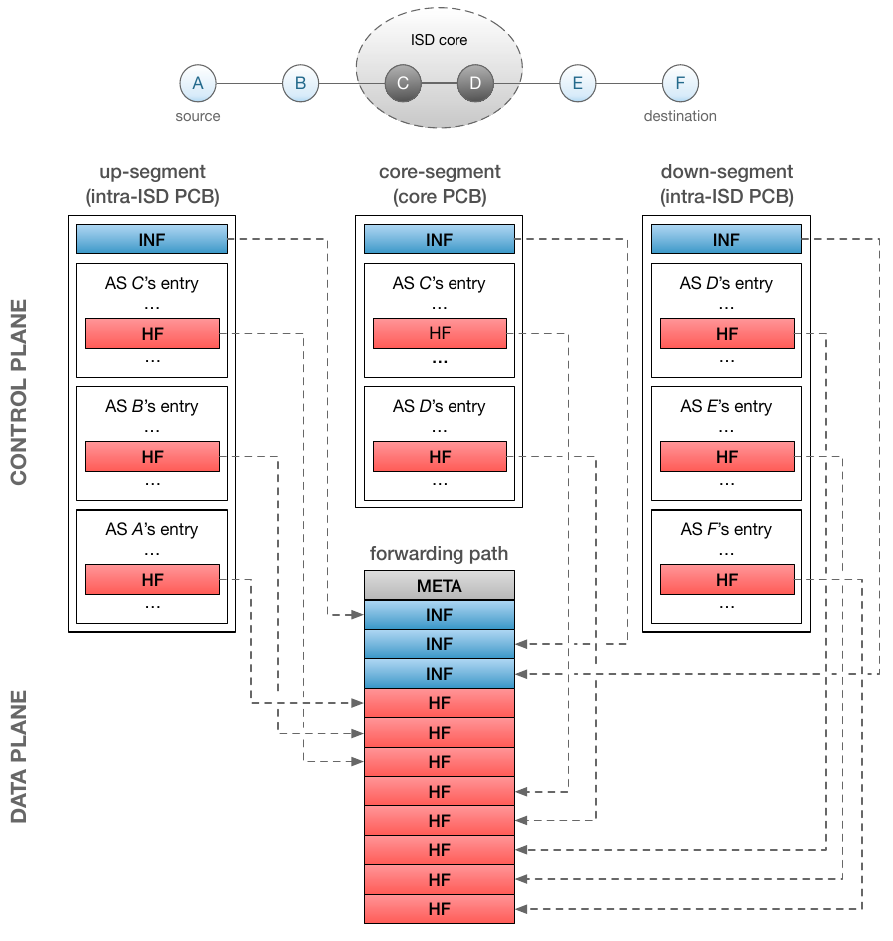
\includegraphics[width=0.75\textwidth]{figures/scion_path_header_construction.png}
    \caption{Construction of the path header out of the path segments. Figure taken from Section 5.4 of the SCION book \cite{Perrig2022}.}
    \label{fig:scion_path_header_contruction}
\end{figure}

When an end host receives a SCION packet, it can use the information in the path header to send a response back to the sender.
In the reply packet, the order of the info and hop fields must be reversed.
Additionally, the $ConsDir$ flag in the info fields has to be flipped, $CurrINF$ and $CurrHF$ should be set to 0, and the order the $SegLen$ fields must be reversed.
This path reversal also allows border routers to communicate any issues encountered during packet processing back to the sender.
Further details on packet processing are explained in the next section.

\subsubsection{Processing at Routers}

The SCION border routers executes various tasks when processing SCION packets and these tasks depend on the position of the router in the path.
The following four router positions are distinguished:

\begin{enumerate}[label=P\arabic*]
    \item In the middle of a path segment and packet transits the AS, i.e. this only needs one hop field.
    \item At the joint of two path segments and packet transfers AS, i.e. this needs two hop fields.
    \item In the source AS.
    \item In the destination AS.
\end{enumerate}

Additionally, the specific tasks performed by the router also depend on whether it is an ingress or egress router of the AS.

The tasks for the ingress border router include:
\begin{enumerate}
    \item Ensure that the interface through which the packet was received matches the interface in the current hop field.
    \item Verify that the hop field is not expired and is within its validity period.
    \item Implicitly determine the position of the router in the path based on the header fields (in case of P1, P2, P4).
    \item Perform some general integrity checks on the packet header.
    \item Only in the cases of P1, P2, and P4, and if ConsDir is zero: XOR the $SegID$ of the current info field with $HFAuth$ of the current hop field, i.e. $SegID := SegID \oplus HFAuth$.
    \item Compute $\sigma$ according to the equation shown in \cref{sec:mac_calc}, by using the $SegID$ of the current info field and verify that it matches the $HFAuth$ of the current hop field.
    \item In case of P2: Verify that the segment combination is valid (for example core to down segment is okay, but core to core is not. Check rules in Table 5.1 in the SCION book \cite{Perrig2022} for a complete list of allowed combination).
    Additionally, increment $CurrHF$ and $CurrINF$ by one and verify the second hop field (steps 2 and 6).
    \item In case of P4: Check that the packet header contains the correct destination ISD and AS identifiers.
    \item Finally, encapsulate the packet and forward it to the egress border router (on the interface specified in the current hop field, in case of P1 and P2) or to the destination host (based on the destination address, in case of P4).
\end{enumerate}


The following tasks have to be performed by the egress border router:
\begin{enumerate}
    \item Decapsulate the SCION packet.
    \item Implicitly determine the position of the router in the path based on the header fields (in case of P1 - P3).
    \item Perform some general integrity checks on the packet header.
    \item Check $HFAuth$ of the current hop field (see steps 2 and 6 in the ingress router tasks).
    \item If router is in position P1-P3 and if $ConsDir$ is one: XOR the $SegID$ of the current info field with $HFAuth$ of the current hop field, i.e. $SegID := SegID \oplus HFAuth$.
    \item Increment $CurrHF$ by one.
    \item Forward the SCION packet to the neighboring AS/router.
\end{enumerate}


If any verification step fails, the router has to drop the packet and inform the sender about the issue by sending a ``parameter problem'' SCMP message back.

Note that the hop field is verified twice in the cases of P1 and P2, once each by the ingress and egress border router.
Although this induces some overhead, it offers several advantages:
The ingress router can drop invalid packets early, thereby conserving forwarding resources.
Validation at the egress router ensures that the packet has not been tampered with during its transit within the AS.


\subsection{Security Mechanisms}
In this section, we will cover the most important security mechanisms in SCION.


\subsubsection{Control Plane PKI (CP-PKI)}
\label{sec:cp_pki}
As mention in the \cref{sec:control_plane}, control plane packets, especially PCB are authenticated and contain a signature.
This authentication relies on the control plane public key infrastructure (CP-PKI) of SCION.
Here, we provide only a brief overview of the CP-PKI; detailed information can be found in Section 3.1 of the SCION book \cite{Perrig2022}.

The root of trust in the CP-PKI is the TRC, which include root certificates.
These are used to verify the certificates of certification authorities (CAs).
CAs issue certificates to ASes, which contain the public key of the AS.
This certificate chain is being used to verify the authenticity of an AS.
Each AS (including its border routers, SCION end hosts etc.) knows the TRC of its ISD and can thus verify the certificates of other ASes within the ISD.
This ensures that only valid and authorized ASes can participate in the SCION network, as PCBs are only accepted if they are signed by a valid AS certificate.

While authentication based on signature and certificates may work well for the control plane with low packet rates, the data plane with high packet rates requires a more efficient authentication mechanism.
This is where the DRKey comes into play, which is explained in the next section.

\subsubsection{Dynamically Recreatable Keys (DRKey)}
\label{sec:drkey}
This section explains the dynamically recreatable key (DRKey) system and its application within SCION.
Since it relies on symmetric cryptographic keys, it is much faster than the CP-PKI.
This allows for efficient packet authentication in the data plane at high bandwidths and mitigates the risk of Denial-of-Service (DoS) attacks that could occur with slower asymmetric cryptography.
Nevertheless, the DRKey system uses CP-PKI to establish the initial keys.

In DRKey, one entity is on the so-called fast side, as it can derive the key quickly based on locally stored secrets.
The other entity, on the slow side, first needs to fetch the key by issuing a request through the control plane.
Which entity is on the fast or slow side depends on the application.
Generally, the more critical side, i.e. the side more exposed to attacks, is on the fast side.
For example, the border router generating an SCMP error message due to a packet processing error is on the fast side, and the source end host receiving the SCMP error message is on the slow side.

Consider the setup depicted in \cref{fig:drkey_setup} where the server $S_B$ is on the fast side and the host $H_A$ on the slow side.
\begin{figure}[h]
    \centering
    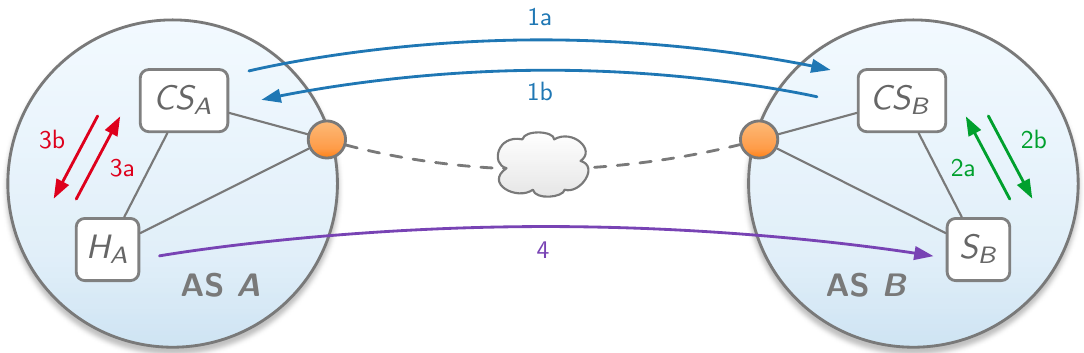
\includegraphics[width=0.75\textwidth]{figures/drkey_topo.png}
    \caption{DRKey communications between an end host and server in different ASes. Based on Figure 3.2 from the SCION book \cite{Perrig2022}.}
    \label{fig:drkey_setup}
\end{figure}

Each AS selects a randomly generated local secret value, $SV_A$ and $SV_B$ respectively, which is shared to trusted entities within the same AS (e.g. the certificate service).
This secret is used together with a pseudo random function (PRF) by the certificate service in AS B $CS_B$ to derive $K_{B \rightarrow A} = \text{PRF}_{SV_B}(A)$.
The arrow notation indicates that $B$ is on the fast side (it can use the local secret to derive it) and $A$ on the slow side (it has to fetch the key from $B$).
The key fetching of $CS_A$ from $CS_B$ is shown by the arrows 1a and 1b in \cref{fig:drkey_setup}.
Arrows 2a and 2b show that server $S_B$ is trusted and can therefore obtain the secret $SV_B$.
When host $H_A$ wants to authenticate itself to server $S_B$ (arrow 4), it contacts the certificate service $CS_A$ and requests a host-to-host key $K_{B:S_B \rightarrow A:H_A}$, which $CS_A$ can locally derive using $K_{B \rightarrow A}$ (arrows 3a and 3b).
Because $S_B$ is on the fast side, it can derive the key $K_{B:S_B \rightarrow A:H_A}$ using $SV_B$.

\subsubsubsection{Key Derivation}
In the following, we will explain the key derivation process in more detail.

Based on the AS-to-AS key $K_{B \rightarrow A}$, second level keys (host-to-AS or AS-to-host) will be derived like this:
\begin{align*}
K_{B \rightarrow A:H_A} &= \text{PRF}_{K_{B \rightarrow A}}(0 \parallel H_A) \\
K_{B:S_B \rightarrow A} &= \text{PRF}_{K_{B \rightarrow A}}(1 \parallel S_B)
\end{align*}

$H_A$ and $S_B$ are the host and server addresses, respectively.
Finally, the third level (host-to-host) key can be derived using the host-to-AS key and by applying the PRF to the slow host's address:
\begin{align*}
    K_{B:S_B \rightarrow A:H_A} = \text{PRF}_{K_{B:S_B \rightarrow A}}(H_A)
\end{align*}

The secrete value $SV$ can be different for different protocols and applications.

\subsubsubsection{SCION Packet Authentication Option (SPAO)}
\label{sec:spao}
One prominent application that uses DRKey is the SCION packet authentication option (SPAO).
SPAO is added to the SCION header of a data plane packet and provides source authentication between end hosts.
Since even the first packet sent is authenticated, there is no need for explicit key exchange between end hosts.
Additionally, SPAO also provides integrity protection of the packet.
To achieve this, different algorithms are supported.
The specific algorithms and further details on SPAO can be found in the SCION book or on the official documentation website \cite{anapayaSCIONPacket}.


\subsection{Anapaya}
In 2017, the demand for commercial usage of SCION increased as several Internet Service Providers (ISPs) and entities in the financial sector wanted to adopt it.
As a result, the company Anapaya Systems was founded by the ETH professors Adrian Perrig, David Basin, and Peter Müller.
Since then, the demand for SCION in the industry has continued to grow.
Interest in SCION extends beyond industry to the academic community as well.
The core SCION components are open source, allowing them to be inspected, tested, and used by anyone.
Other components, such as a management system, are exclusively distributed to Anapaya customers \cite{ethzSecureInternet}.

The Cyber-Defense Campus is also a customer of Anapaya and uses SCION for their research.
Further details on their SCION network setup can be found in \cref{ch:methodology}


\section{Security Testing}
\label{sec:security_testing}
Regular security tests are essential to ensure the security of a system.
This is especially important for systems that are exposed to the Internet, as they face a high risk of being attacked.
By proactively testing the security of a system, vulnerabilities can be identified and fixed before they are exploited by attackers.
In the following, we will provide a general overview of different security testing methods and tools.

\subsection{Automatic Scanning Tools}
Automatic scanning tools offer an easy and efficient method to identify vulnerabilities and misconfiguration of specific software, entire networks or even individual devices.

When scanning devices, many tools are capable of performing both unauthenticated and authenticated scans.
Authenticated scans, which use credentials to log in to the target device, can gather more detailed information about the device and provide more accurate results.
At the end of a scan, these tools generate reports that offer a comprehensive overview of the identified vulnerabilities and weaknesses.
Some tools even provide suggestions for remediation.
Examples of automatic scanning tools include Nessus \cite{nessus} and OpenVAS \cite{openvas}.
The primary difference between these tools is that Nessus is a proprietary, while OpenVAS is open-source.
Both tools are free to use; however, the paid version of Nessus additionally offers the option to run compliance scans.
Compliance scan checks if the target device adheres to specific standards, such as the Center for Internet Security (CIS) benchmarks.

Other tools, such as SSH audit \cite{sshaudit}, focus on specific services, in this case SSH.
They check the configuration of the service and provide recommendations for improving its security.


\subsection{Manual Testing}
Manual testing is a more time-consuming and complex process compared to automatic scanning tools.
While automatic tools provide a good overview of known vulnerabilities and misconfiguration, manual testing can identify more complex issues that are not easily detectable or even not possible to detect by automatic tools.
These include logical errors, custom software, complex setups, dependencies between different systems, and other issues that require human intelligence to find.
This human expertise can uncover subtle weaknesses and nuances in different environments that automated tests might miss.

